\documentclass{article}
\usepackage{amsmath}
\usepackage{pgfplots}
\usetikzlibrary{external}
\tikzexternalize
\tikzset{external/system call={latex \tikzexternalcheckshellescape
  -halt-on-error -interaction=batchmode -jobname "\image" "\texsource";
  dvips -o "\image".eps "\image".dvi}}
\begin{document}
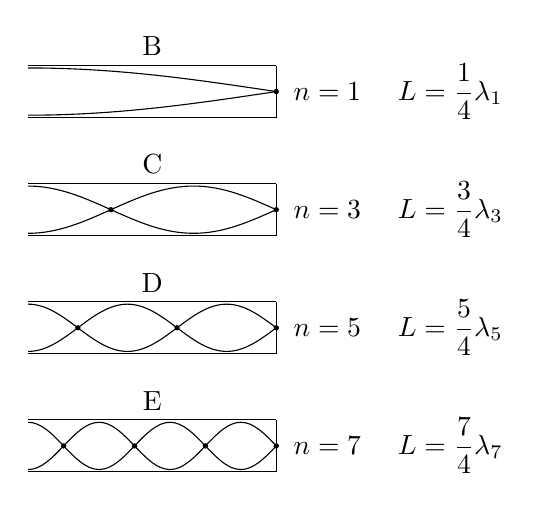
\begin{tikzpicture}[scale=0.3]
\draw (0,1.1) -- (10.5,1.1) node[midway,above] {B}; %top
\draw (0,-1.1) -- (10.5,-1.1); %bottom
\draw (0,-1) cos (10.5,0); %top curve
\draw (0,1) cos (10.5,0); %bottom curve
\draw (10.5,1.1) -- (10.5,-1.1) node[midway,anchor=west] {\;$n=1$ \quad $L=\dfrac{1}{4}\lambda_{1}$}; %right
\draw[fill=black] (10.5,0) circle (2.5pt); %circle
\begin{scope}[yshift=-5cm]
\draw (0,1.1) -- (10.5,1.1) node[midway,above] {C}; %top
\draw (0,-1.1) -- (10.5,-1.1); %bottom
\draw (0,1) cos (3.5,0) sin (7,-1) cos (10.5,0); %top curve
\draw (0,-1) cos (3.5,0) sin (7,1) cos (10.5,0); %bottom curve
\draw (10.5,1.1) -- (10.5,-1.1) node[midway,anchor=west] {\;$n=3$ \quad $L=\dfrac{3}{4}\lambda_{3}$}; %right
\draw[fill=black] (3.5,0) circle (2.5pt); %circle
\draw[fill=black] (10.5,0) circle (2.5pt); %circle
\end{scope}
\begin{scope}[yshift=-10cm]
\draw (0,1.1) -- (10.5,1.1) node[midway,above] {D}; %top
\draw (0,-1.1) -- (10.5,-1.1); %bottom
\draw (0,1) cos (2.1,0) sin (4.2,-1) cos (6.3,0) sin (8.4,1) cos (10.5,0); %top curve
\draw (0,-1) cos (2.1,0) sin (4.2,1) cos (6.3,0) sin (8.4,-1) cos (10.5,0); %bottom curve
\draw (10.5,1.1) -- (10.5,-1.1) node[midway,anchor=west] {\;$n=5$ \quad $L=\dfrac{5}{4}\lambda_{5}$}; %right
\draw[fill=black] (2.1,0) circle (2.5pt); %circle
\draw[fill=black] (6.3,0) circle (2.5pt); %circle
\draw[fill=black] (10.5,0) circle (2.5pt); %circle
\end{scope}
\begin{scope}[yshift=-15cm]
\draw (0,1.1) -- (10.5,1.1) node[midway,above] {E}; %top
\draw (0,-1.1) -- (10.5,-1.1); %bottom
\draw (0,1) cos (1.5,0) sin (3,-1) cos (4.5,0) sin (6,1) cos (7.5,0) sin (9,-1) cos (10.5,0); %top curve
\draw (0,-1) cos (1.5,0) sin (3,1) cos (4.5,0) sin (6,-1) cos (7.5,0) sin (9,1) cos (10.5,0); %bottom curve
\draw (10.5,1.1) -- (10.5,-1.1) node[midway,anchor=west] {\;$n=7$ \quad $L=\dfrac{7}{4}\lambda_{7}$}; %right
\draw[fill=black] (1.5,0) circle (2.5pt); %circle
\draw[fill=black] (4.5,0) circle (2.5pt); %circle
\draw[fill=black] (7.5,0) circle (2.5pt); %circle
\draw[fill=black] (10.5,0) circle (2.5pt); %circle
\end{scope}
\end{tikzpicture}
\end{document}

